\section{Limitations} \label{sec:limitations}
In this section we will present the main limitation of the developed system, mainly in the software components.
Most of these limitations exist due to development choices and not due to any particular impediment from realising them.
The main reasons that led us to make such choices include, but are not limited to, the project development being done by a single person, limited development time and, most importantly, the fact that the entire project has been developed from a home environment during the Portuguese COVID-19 lock-downs in early 2021.

% Hardware
\subsection{Hardware}
For the most part, the hardware components were chosen in a way they would not pose a big obstacle to the development of more advanced demonstration concepts.
Regardless, the designed and 3D-printed motor support was mostly meant to allow the motor to function properly without the user having to hold on to it.

This was one of the limitations that rose from developing the project from a home environment, where the development of the 3D model had to be done in an open-loop situation, without any feedback or preliminary testing before sending the complete design for production.
Ultimately this meant one of the 3D printed pieces was defective but, luckily, the problem was lessened with some hot glue, as seen in \autoref{fig:hotglue-support} (page \pageref{fig:hotglue-support}).

\begin{figure}[t]
	\centering
	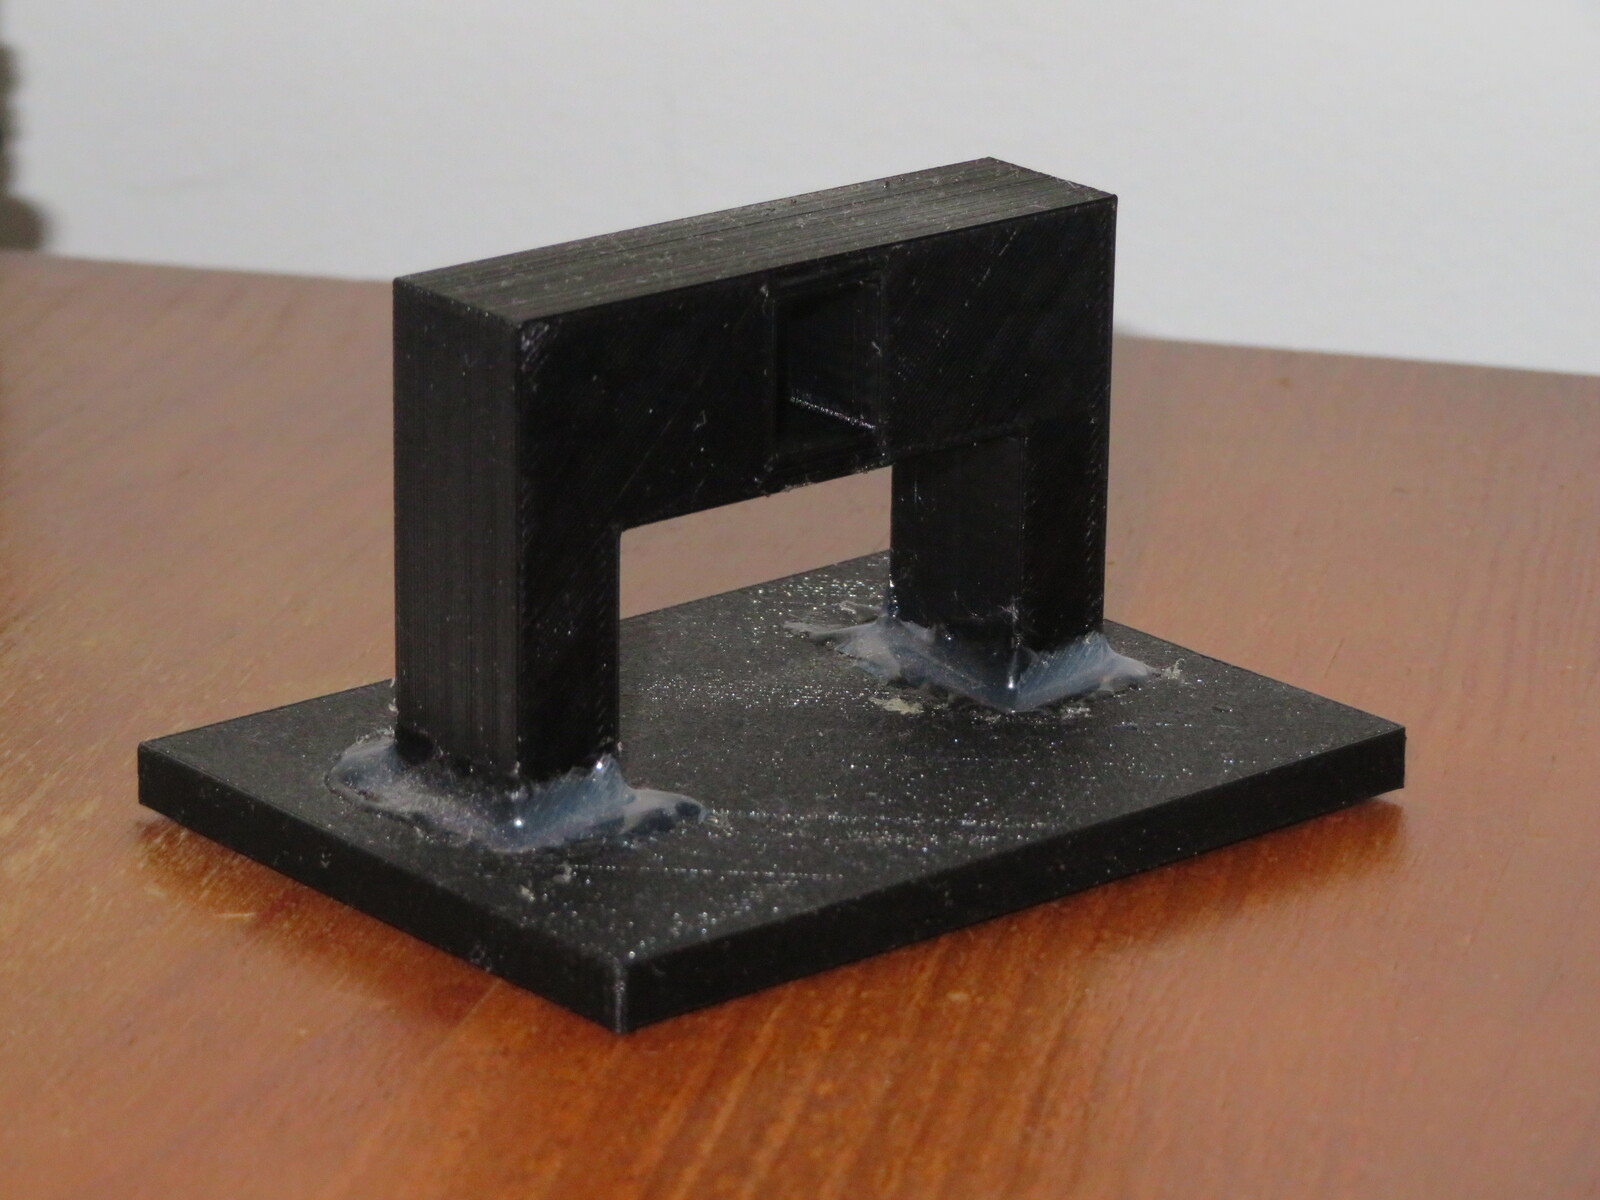
\includegraphics[width=0.8\linewidth]{IMG_3044_resized.JPG}
	\caption{3D printed support, fixed with hot glue}
	\label{fig:hotglue-support}
\end{figure}

Another hardware aspect that could be considered a limitation is the small encoder resolution (12 PPR).
This has not impacted the performance because the motor's gearbox, with a reduction ratio of $30:1$, makes the motor + gearbox + encoder set have an apparent 360 PPR encoder on the output shaft.
As we are only interested in controlling said output shaft, the actual (virtual) encoder resolution is more than enough for a proof-of-concept system.
% Maybe talk about the 32-byte I/O from the communication board?

